%-------------------------------------------------------------------------------
\begin{frame}[label=overview]{Overview}
  \tableofcontents
\end{frame}
%===============================================================================
\section{Introduction}
%-------------------------------------------------------------------------------
\begin{frame}{What is \LaTeX? A typesetting program}
  \centering\pause
  \begin{tikzpicture}[x=.5\textwidth,y=.5\textwidth]
    \visible<2->{
      \node (i) at (0,0) {\frame{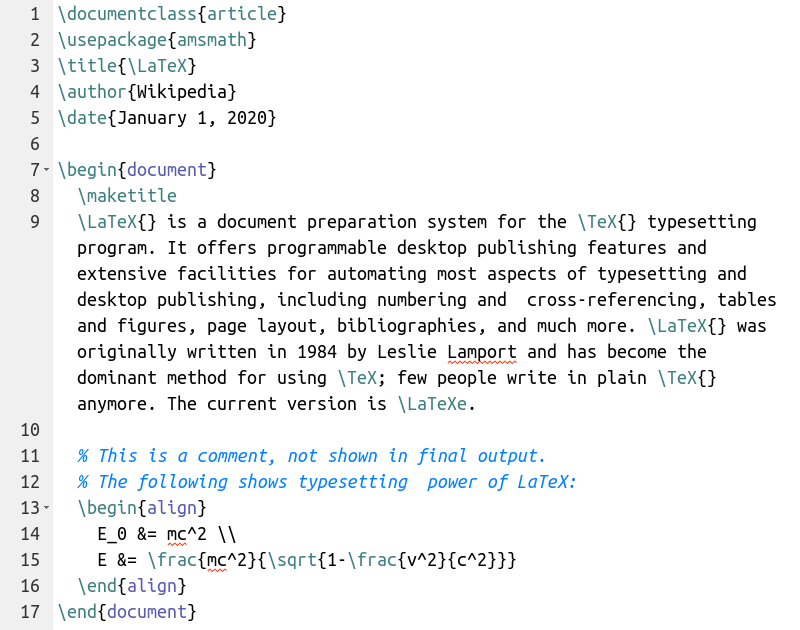
\includegraphics[width=.4\linewidth]{tex-in}}};
      \node[above] at (i.north) {input: \texttt{filename.tex}}; }
    \visible<4->{
      \node (o) at (1,0) {\frame{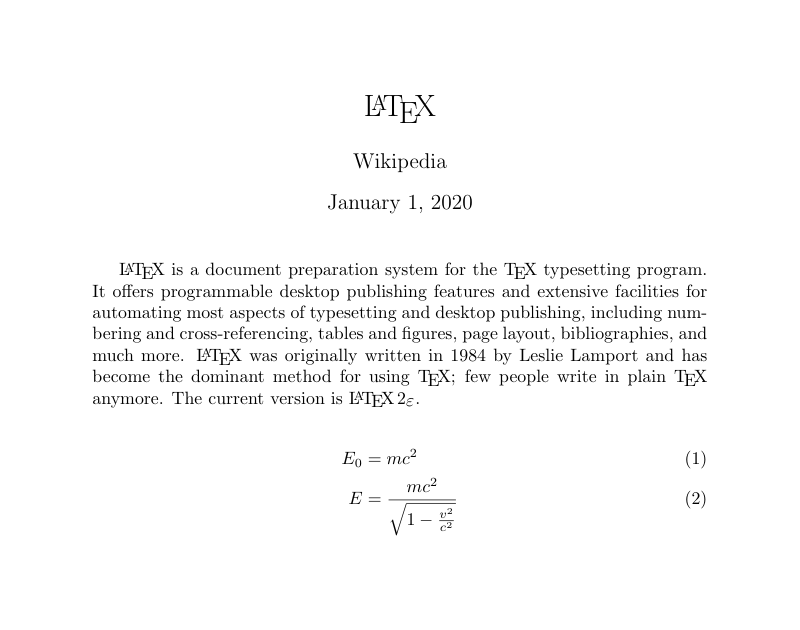
\includegraphics[width=.4\linewidth]{tex-out}}};
      \node[above] at (o.north) {output: \texttt{filename.pdf}}; }
    \visible<3->{\node[align=center] at (.5,0) {\textcolor{c1}{\LaTeX}\\\huge\rarr}; }
  \end{tikzpicture}
\end{frame}
%-------------------------------------------------------------------------------
\begin{frame}{Advantages + Disadvantages}
\pbox{\paragraph{Advantages}
  \begin{itemize}
    \item plain-text editing
    \item automate counters, cross-references, \dots
    \item beautiful math + vector graphics
    \item version control
    \item free + open source
  \end{itemize}}
\pbox{\paragraph{Disadvantages}
  \begin{itemize}
    \item learning curve
    \item co-authors + comments
    \item not WYSIWYG\\\emph{what you see is what you get}
    \item tables = pain
  \end{itemize}}
\end{frame}
%-------------------------------------------------------------------------------
\begin{frame}{\LaTeX\ vs MS Word}
  \centering
  \begin{tikzpicture}[x=.6\linewidth,y=.3\linewidth,>=latex]
    \draw[<->] (1,0) -- node[below] {Document Complexity + Size}
               (0,0) -- node[above,rotate=90] {Effort + Time} (0,1);
    \draw[thick,color=c2,domain=0:.5,samples=256] plot ({\x,4*\x^2}) node[right]{MS Word};
    \draw[thick,color=c1,domain=0:.9,samples=256] plot ({\x,sqrt(\x)}) node[right]{\LaTeX};
  \end{tikzpicture}
\end{frame}
%===============================================================================
\section{How \LaTeX\ Works}
%-------------------------------------------------------------------------------
\begin{frame}[fragile]{3 Layers of \LaTeX}
\newcommand{\layer}[1]{\pbox[.16]{\textbf{#1}}}
  \begin{enumerate}
    \item  \layer{``kernel''}      parses code, stores data, creates PDF
    \item[]\layer{+ ``built-ins''} functions, \eg \lstinline|\newcommand{\pie}{3.14}|;
                                   then \lstinline|\pie| becomes ``3.14''
    \item  \layer{``classes''}     types of document, \eg an article, having: format, title, etc.
    \item[]\layer{+ ``packages''}  modify or extend a class, \eg adding graphics
    \item  \layer{``document''}    this specific document, \eg your thesis
  \end{enumerate}
\end{frame}
%-------------------------------------------------------------------------------
\begin{frame}[fragile]{Kernel: Putting Stuff on a Page}
\newcommand{\bfbox}[1]{\sbox0{#1}%
  {\color{c2!33}\vrule width\wd0 height\ht0 depth\dp0}%
  \llap{\color{c2}\vrule width\wd0 height.05ex depth.05ex}%
  \llap{\usebox0}}%
  \pbox[.5]{
  \paragraph{Boxes:}
  letters \rarr words \rarr lines\\
  \null\quad\rarr paragraphs \rarr pages
  \bigskip\paragraph{Combining Boxes:}
  \begin{itemize}
    \item \textbf{modes:} horizontal, vertical, math
    \item \textbf{glue:} stretchy space
    \item \textbf{floats:} ``float'' around (figures/tables)
    \item \textbf{penalties:} avoid ``bad'' layouts
  \end{itemize}\medskip}
  \scalebox{2.5}{\colorbox{g}{\pbox[.18]{\itshape
    \bfbox{the} \bfbox{quick} \bfbox{brown} \bfbox{fox}
    \bfbox{jumps} \bfbox{over} \bfbox{the} \bfbox{lazy} \bfbox{dog}
  }}}
\end{frame}
%===============================================================================
\section{Getting Started}
%-------------------------------------------------------------------------------
\begin{frame}{Editors}
\pause
\pbox{
\includegraphics[height=5ex]{overleaf}
  \begin{itemize}
    \item no install + package management
    \item must have internet connection
    \item pay to integrate reference database
    \item some collaborate features
    \item limited hotkeys
  \end{itemize}}
\pause
\pbox{\foreach \edit in {texstudio,vim,emacs,sublime,vscode}{
  \includegraphics[height=6ex]{\edit}}
  \begin{itemize}
    \item install + manage packages locally
    \item no internet connection required
    \item free to integrate reference database
    \item DIY collaborate
    \item custom hotkeys
  \end{itemize}}
\end{frame}
%-------------------------------------------------------------------------------
\begin{frame}[fragile]{Your First Document}
  \begin{lstlisting}
\documentclass{article}
% document header
\begin{document}
  % document body
  Hello World
\end{document}
  \end{lstlisting}
\end{frame}
%-------------------------------------------------------------------------------
\begin{frame}{Document Elements}
  \begin{itemize}
    \item title, author, date
    \item sections, subsections, etc.
    \item math
    \item floats: figures \& tables
    \item cross-references \& table of contents
    \item citations \& bibliography
  \end{itemize}
\end{frame}
%===============================================================================
\section{Resources}
%-------------------------------------------------------------------------------
\begin{frame}[fragile]{Helpful Resources}
\newcommand{\linkbox}[2]{\pbox[.25]{\hrefc{#1}{#2}}}
  \begin{itemize}
    \item \linkbox{https://www.overleaf.com/learn}{Learn LaTeX}
      a great resource for learning LaTeX
    \item \linkbox{https://www.overleaf.com}{Overleaf}
      online \LaTeX\ writing application
    \item \linkbox{https://www.latex-tutorial.com/installation}{\LaTeX\ Install Guide}
      to install \LaTeX\ on your computer (offline)
    \item \linkbox{https://www.texstudio.org}{TeXstudio}
      \LaTeX-specific code editor (offline)
    \item \linkbox{https://tex.stackexchange.com}{\TeX\ Stack Exchange}
      Q \& A style how-to and debugging help
    \item \linkbox{https://tikz.dev}{Ti\textit{k}Z Manual}
      documentation for drawing diagrams
    \item \linkbox{https://github.com/jessexknight/latex}{Github Repository}
      example documents \& ``cheat sheets''
  \end{itemize}
\end{frame}
%-------------------------------------------------------------------------------
\begin{frame}[fragile]{Notable \TeX\ Stack Exchange Questions}
\newcommand{\tselink}[2]{\hrefc{https://tex.stackexchange.com/questions/#1}{#2}}
  \begin{itemize}
    \item \tselink{339}{Which editors can I use to write \LaTeX?}
    \item \tselink{14}{How do I write the symbol \dots}
    \item \tselink{595}{How can I make bold math symbols?}
    \item \tselink{39017}{How to influence the position of figures and tables?}
    \item \tselink{25701}{What are \texttt{bibtex} vs \texttt{biber} and \texttt{biblatex} vs \texttt{natbib}?}
    \item \tselink{246}{What do \texttt{\string\include} vs \texttt{\string\input} do?}
    \item \tselink{8351}{What do \texttt{\string\makeatletter} and \texttt{\string\makeatother} do?}
    \item \tselink{1319}{How can I flex on Word plebs?}
  \end{itemize}
\end{frame}
